\chapter{Introduction}
\label{cha:Introduction}

Pose and motion estimation of objects is an active field of research due to the growing digitalization of day-to-day processes. A vast majority of existing pose estimation methods take advantage of sensors and markers as indicators for joints. Additionally, the rigid parts of an object and its joints are already known. However, unsupervised methods that are completely independent of user input and detect the pose of an unknown object, constitute a great challenge. Among those methods, the non-rigid registration (see section \ref{nonrigidregistration}) is a well-known approach \cite{survey}.

\begin{figure}[htbp]
	\centering\small
	\begin{tabular}{cc}
		\fbox{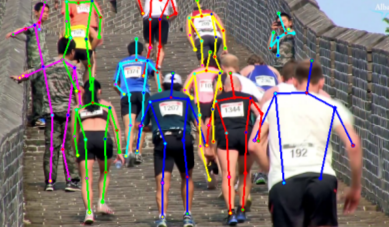
\includegraphics[width=0.43\textwidth]{poseEstimation}} &		% JPEG file
		\fbox{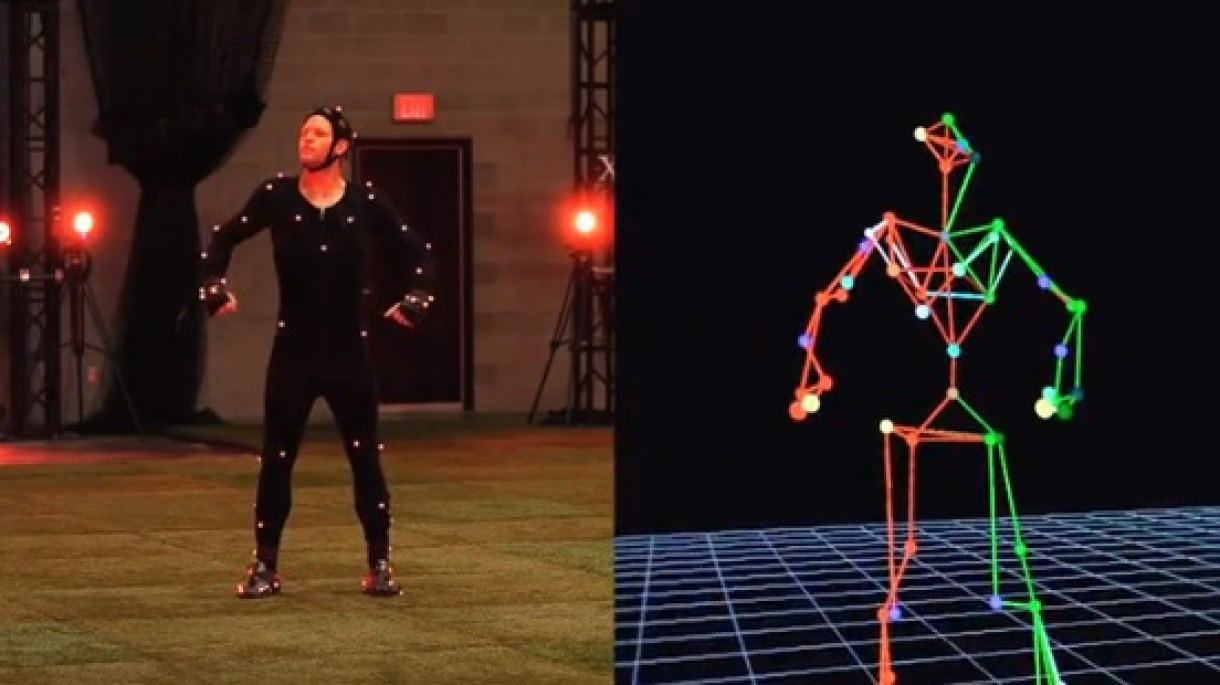
\includegraphics[width=0.45\textwidth]{motionCapture}} 
		\\	% PNG file
		(a) & (b) 
	\end{tabular}
	\caption{Multi-person pose estimation~(a) \cite{poseEstimation} and optical Motion Capture with markers~(b) \cite{MotionCapture}.} 
	\label{fig:motivation}
\end{figure}

\section{Initial idea}
%
% ToDo: Write down use case!
%
The initial project idea was to create a tool for 3D animation purposes using a small puppet to capture its poses in real-time. However, the idea addressed many different challenges, like 3D reconstruction, segmentation, joint and skeleton estimation as well as creating an interface with a 3D animation program. As the implementation of these tasks would go beyond the scope of a thesis project, it was indispensable to break it down into its main areas.  
%TODO: - good structur: what is the problem? What has been done? --> other papers Quickly get to the problem

\section{Main considerations}
To take the puppet pose capture as occasion, following considerations have to be done:
%%
\begin{itemize}
	\item How and in which form is the input data (puppet) received?
	\item What are the rigid parts of the puppet?
	\item What are the joints of the puppet?
	\item Which joints/rigid parts correspond to each other in two different poses?	
\end{itemize}
%%
To answer those questions extensive research has been conducted on pose estimation to get an idea of the general workflow (see section \ref{PoseCapture}), possible difficulties and potential approaches (see chapter \ref{cha:RelatedWork}). Thereby, the main issue of segmenting an articulated object into its rigid part frequently emerged and for this reason the thesis project focuses on this field.

\section{General pose capture workflow}
\label{PoseCapture}
Generally, there are two major steps to capture the pose of an object. First, the object has to be digitalized, which is achieved by a 3D scanning and reconstruction approach. The data might be in form of a point cloud or voxels depending on the reconstruction method (see section \ref{sec:reconstruction}). The second major step includes the analysis of the data to recognize body parts and subsequently joints and if required the skeleton. Depending on the chosen approach, which is usually a segmentation step (see section \ref{sec:segmentation}), there might be a subdivision into sub steps.
%
%TODO: new image with puppet! --> picture, point cloud, skeleton
%
\begin{figure}
	\centering
	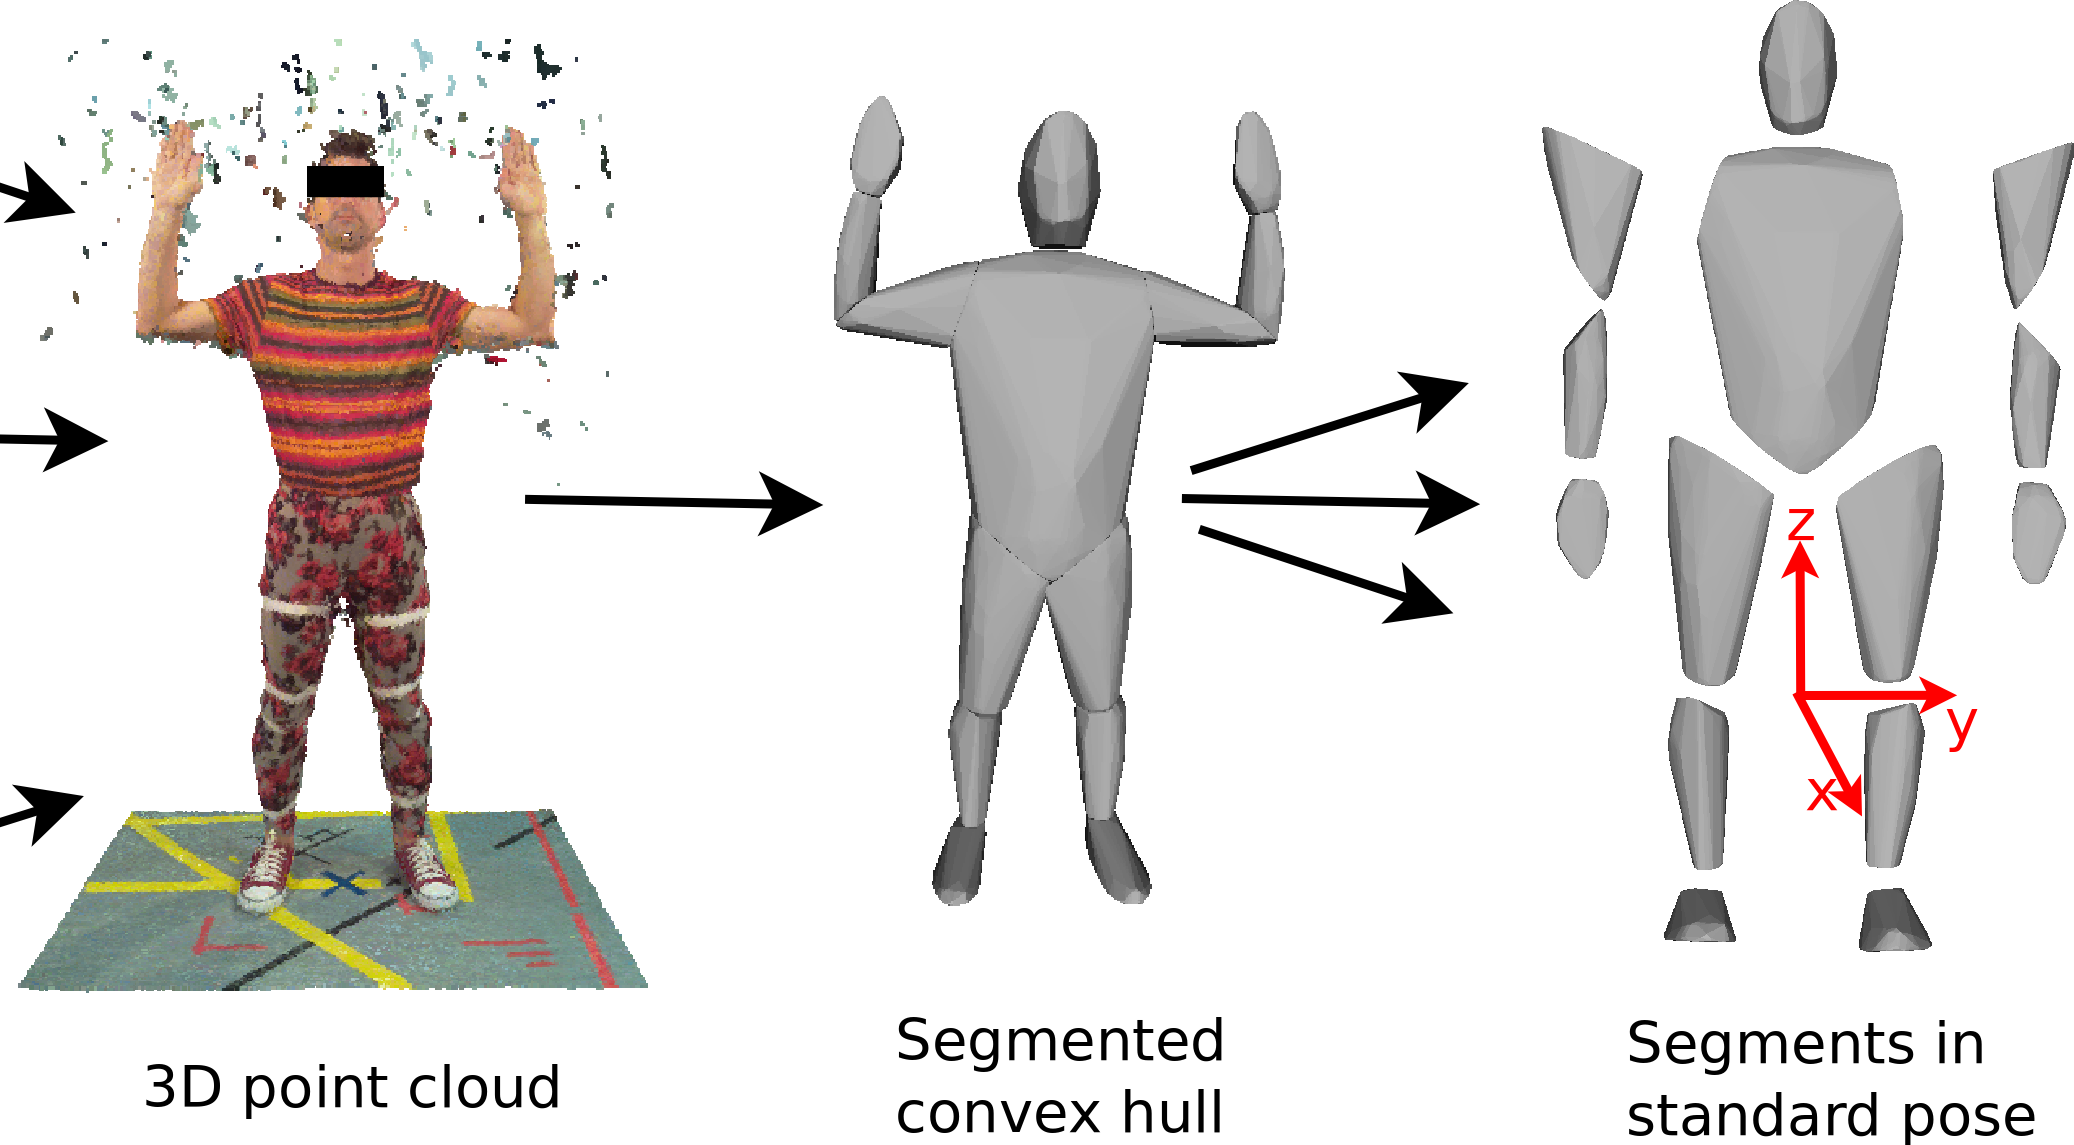
\includegraphics[width=0.7\linewidth]{reconstructionWorkflow}
	\caption{General approach to estimate the pose of a real object, including 3D scanning and reconstruction, 3D segmentation to get the joints and subsequently skeleton extraction}
	\label{fig:posecapture}
\end{figure}
%
\subsection{3D Scanning/Reconstruction}
\label{sec:reconstruction}
%
% ToDo: explain in detail
%
Scanning means collecting a real shape as 3D data. Reconstruction means the approach to convert the raw data to a mesh or process the input data.

Voxelization, Shape from Shilouette, Shape from Shading, Depth camera, stereo camera
%
%TODO: add references
%
\subsection{3D Segmentation}
\label{sec:segmentation}
%
% ToDo: explain methods in detail
% 1) markers/sensors/exoskeleton
% 2) markerless methods
%
How it is done: markers, sensors, shape fitting (already known)
Cite all papers (Voxelization, ....). There are previous approaches with markers and sensors which will not be treated in this work in detail, as markerless options are taken as focus.

\subsubsection{Supervised methods}
Many already existing methods don't require markers and sensors but already assume or know the hierarchical structure or the body parts of the object to be captured (see \cite{multiLayerSkeleton}, \cite{baker2005shape}, \cite{de2008hierarchical} and \cite{michoud2007real}).

\subsubsection{Unsupervised methods}
Although the approaches mentioned in section \ref{sec:currentApproaches} work quite well depending on the application, improvements can be made that are more independent from user inputs.... which leads us to the non-rigid registration \ref{nonrigidregistration}.

\section{Non-rigid registration}
\label{nonrigidregistration}

Generally, registration means the alignment of rigid point clouds (see figure \ref{fig:registration}). A well-known approach to achieve this, is the iterative closest point (ICP) \cite{ICP}, which requires the input point clouds to be aligned quite similar to avoid a local optimum. After registration, a matching error $e$ is achieved, which states the total euclidean distance between the associated points of the registered point clouds. In case of two non-rigid objects (e.g. a human in different poses which is composed of rigid parts) the ICP won't lead to a satisfying registration as associated parts are transformed differently. In order to register a non-rigid object, a segmentation into its rigid parts is required.

\subsection{Prerequisites}
\label{prerequisites}
Assuming, a 3D reconstructed model in form of a point cloud is already available to fully focus on the segmentation of an articulated object in form of a mesh into its rigid parts.

%TODO: Write start position

\subsection{Challenges}
\label{Challenges}
There are many challenges regarding the non-rigid registration of point clouds in 2D, as well as in 3D. First off, the input data can be noisy by means of points not belonging to the object. Furthermore, the approach is computationally expensive and time-consuming, as the corresponding body parts of two meshes need to be detected iteratively. Additionally, the inevitable difficulty of finding the global optimum, related to ambiguous body parts, has to be overcome.

\begin{figure}[H]
	\centering\small
	\begin{tabular}{cc}
		\fbox{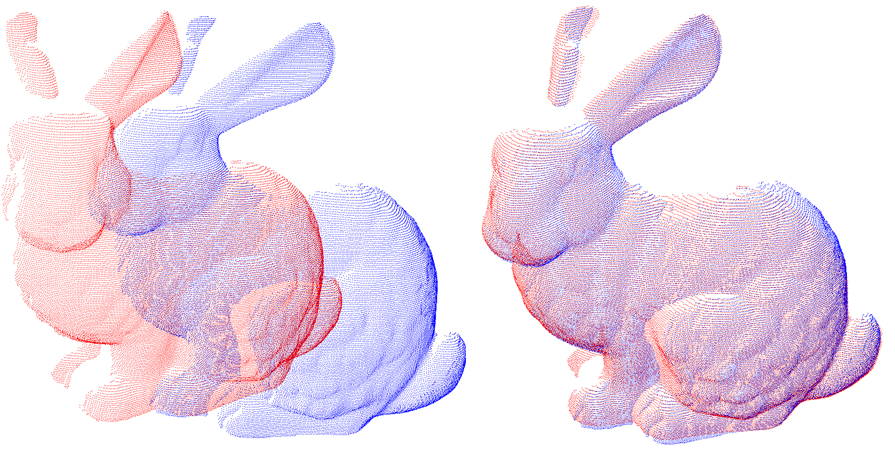
\includegraphics[width=0.43\textwidth]{stanfordBunny}} &		% JPEG file
		\fbox{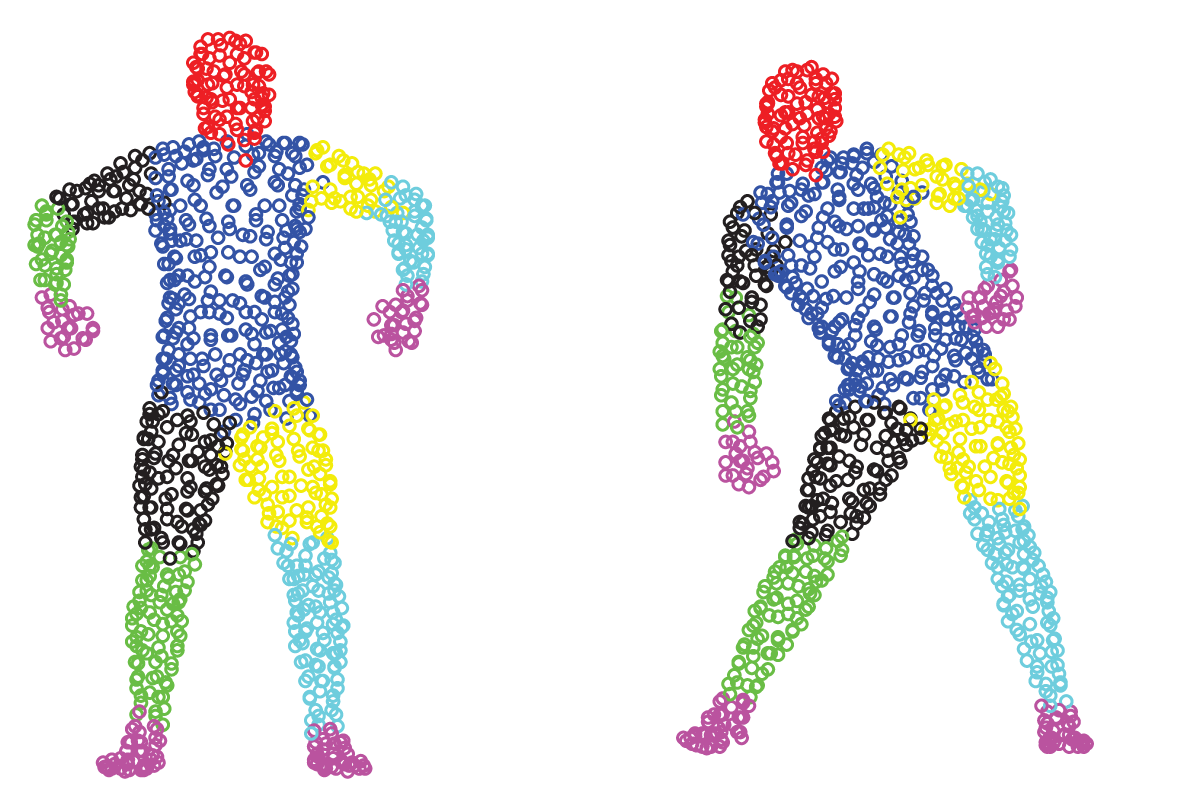
\includegraphics[width=0.45\textwidth]{nonrigidregistration}} 
		\\	% PNG file
		(a) & (b) 
	\end{tabular}
	\caption{Rigid registration of the stanford bunny~(a) \cite{stanfordBunny} and non-rigid registration of a human~(b) \cite{registrationHuman} by detecting its rigid parts.}
	
	\label{fig:registration}
\end{figure}\textbf{}

\section{Related work}
\label{sec:RelatedWork}

By focusing on approaches computing the segmentation of articulated objects from 3D data, many different ones could be detected. They face similar challenges (see subsection \ref{Challenges}) but solve them in different ways
%%
\subsection{Correlated Correspondence}

A main approach for non-rigid registration is proposed by Anguelov \cite{Anguelov04} applying the correlated correspondence algorithm \cite{CorrelatedCorrespondance}. The algorithm takes a \textit{template} Mesh $D_0$ and other Meshes $D_1,\ldots,D_n$ in different configurations as input. The algorithm then performs a probabilistic framework and Expectation-Maximization (EM) to iterate between finding a decomposition of the \textit{template} into rigid parts and detecting them in the other meshes. Furthermore, a random clustering is applied to facilitate the detection of associated rigid parts.
%%
\begin{figure}
	\centering
	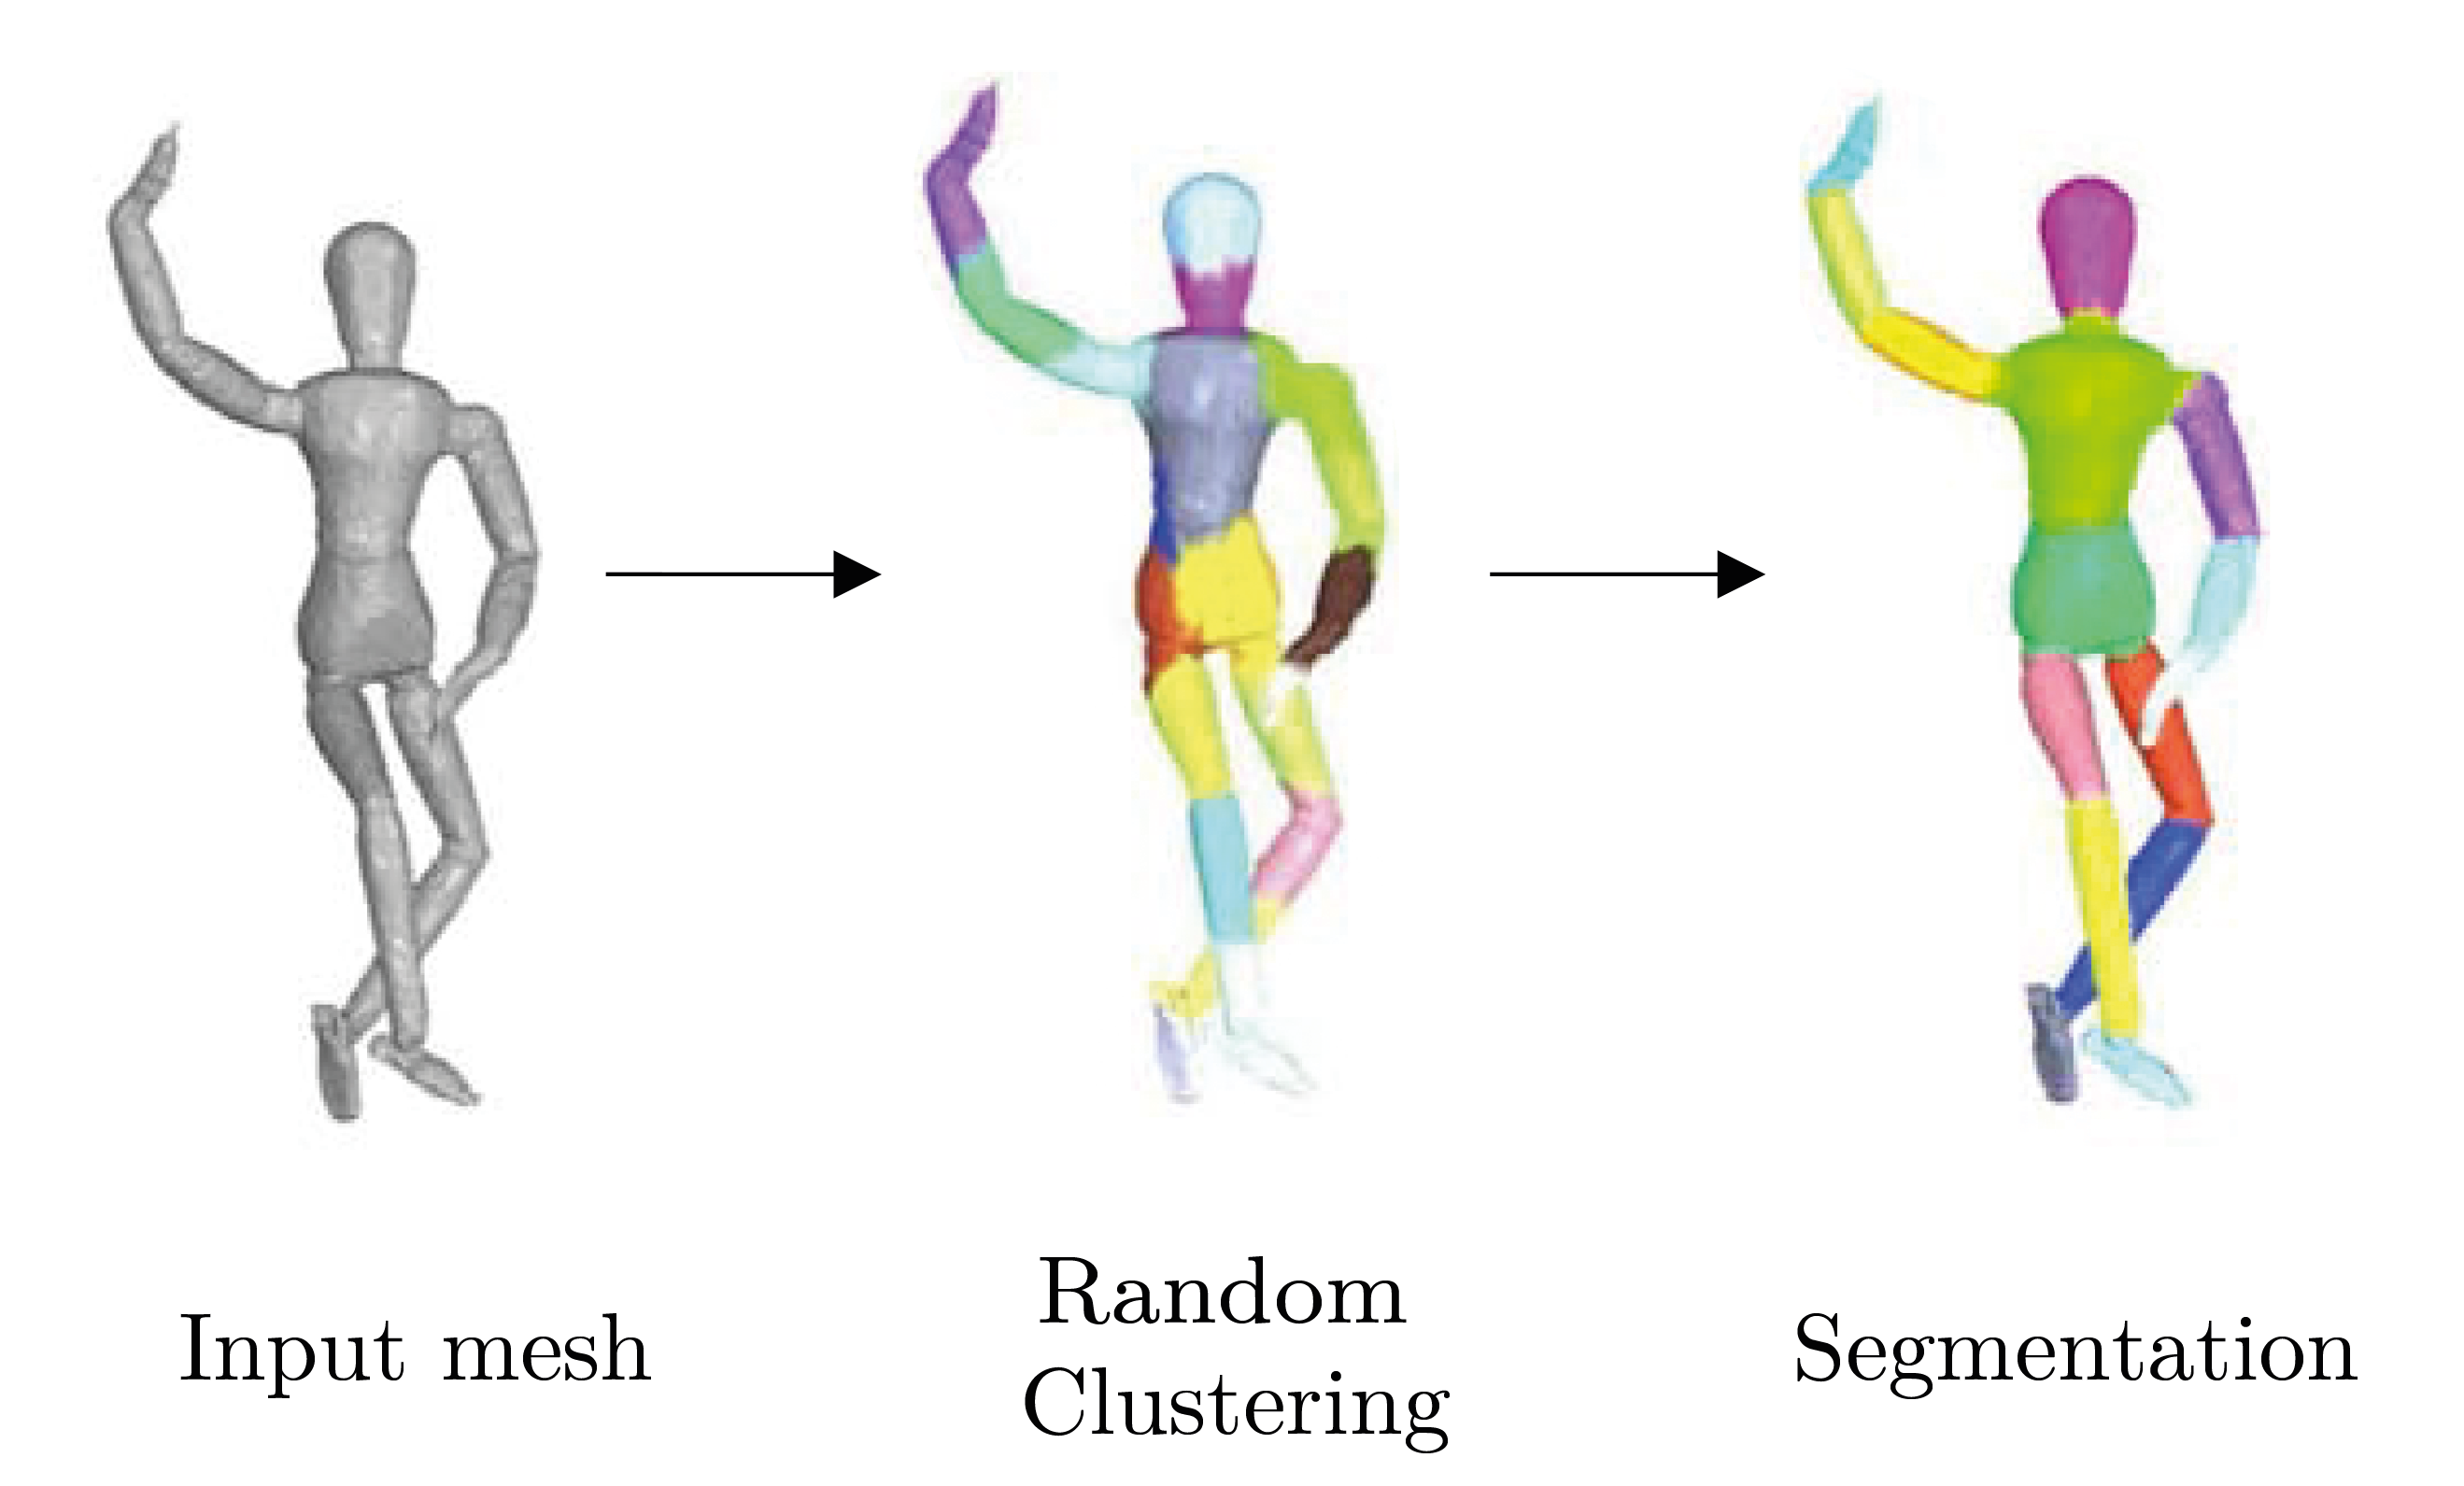
\includegraphics[width=0.7\linewidth]{anguelov}
	\caption{Segmentation a template mesh $M$ into its rigid parts by applying random clustering and a probabilistic framework to iteratively detect associating parts in another mesh \cite{Anguelov04}.}
	\label{fig:correlatedcorrespondance}
\end{figure}
%%
A different approach proposes the recursive detection of body parts by the LRP -- ``largest rigid part'' algorithm \cite {guo2016correspondence}. 
%%
\subsection{LRP}
The LRP algorithm discovers the articulated parts of two objects in different configurations by initially detecting the largest rigid part. This would be the biggest point cluster by applying a single rigid transformation. To reach that, sparse correspondences in combination with RANSAC are implemented. From there, the linking parts are recursively detected by growing clusters from the LRP and reapplying the algorithm. 
%%
\begin{figure}[H]
	\centering\small
	\begin{tabular}{cc}
		\fbox{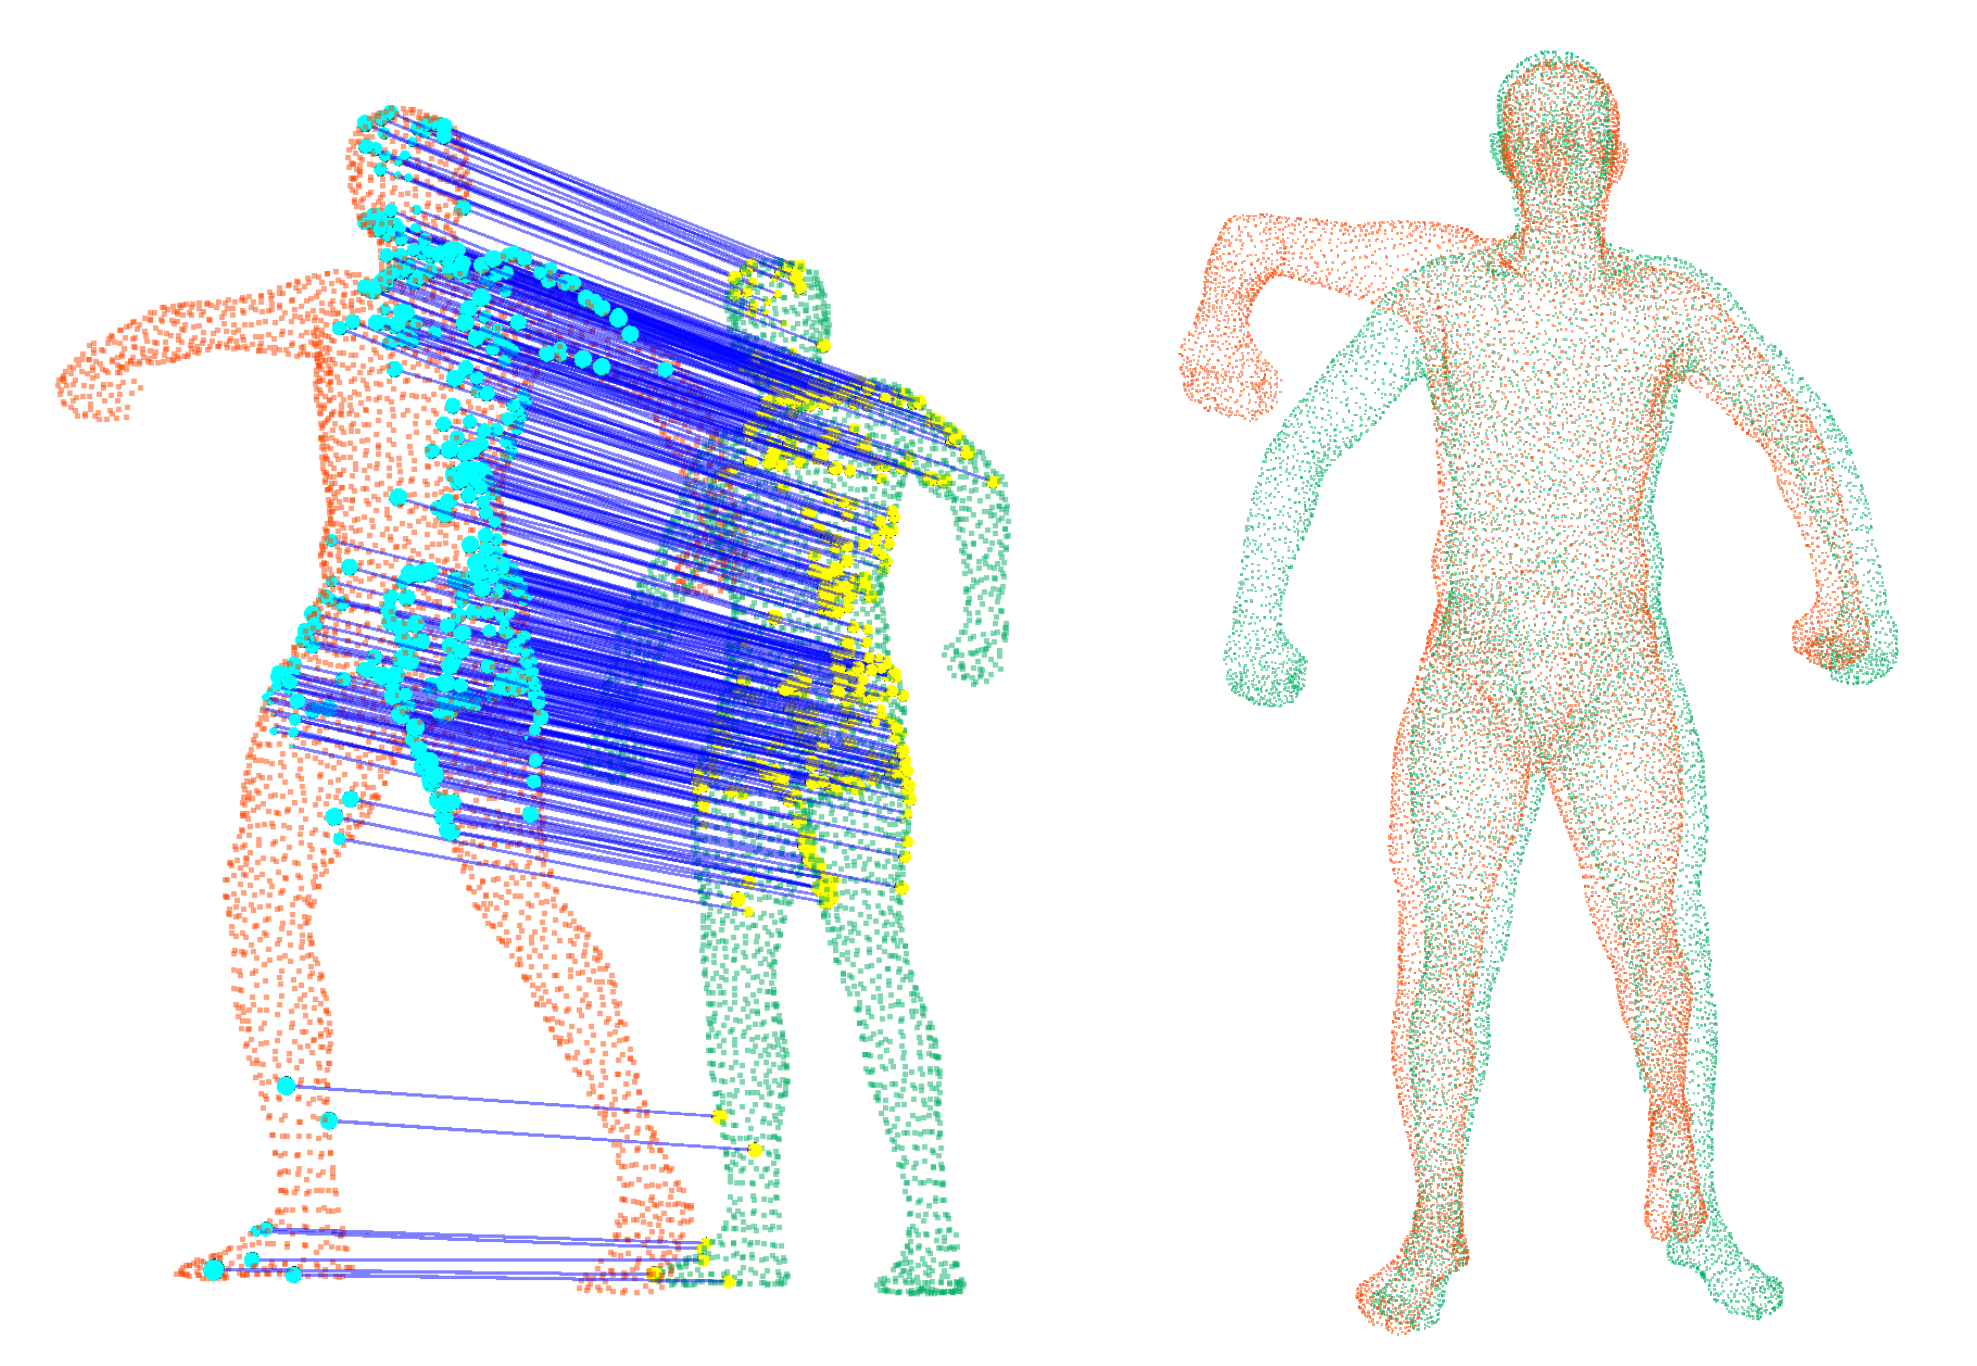
\includegraphics[width=0.45\textwidth]{LRP_body}} &	
		\fbox{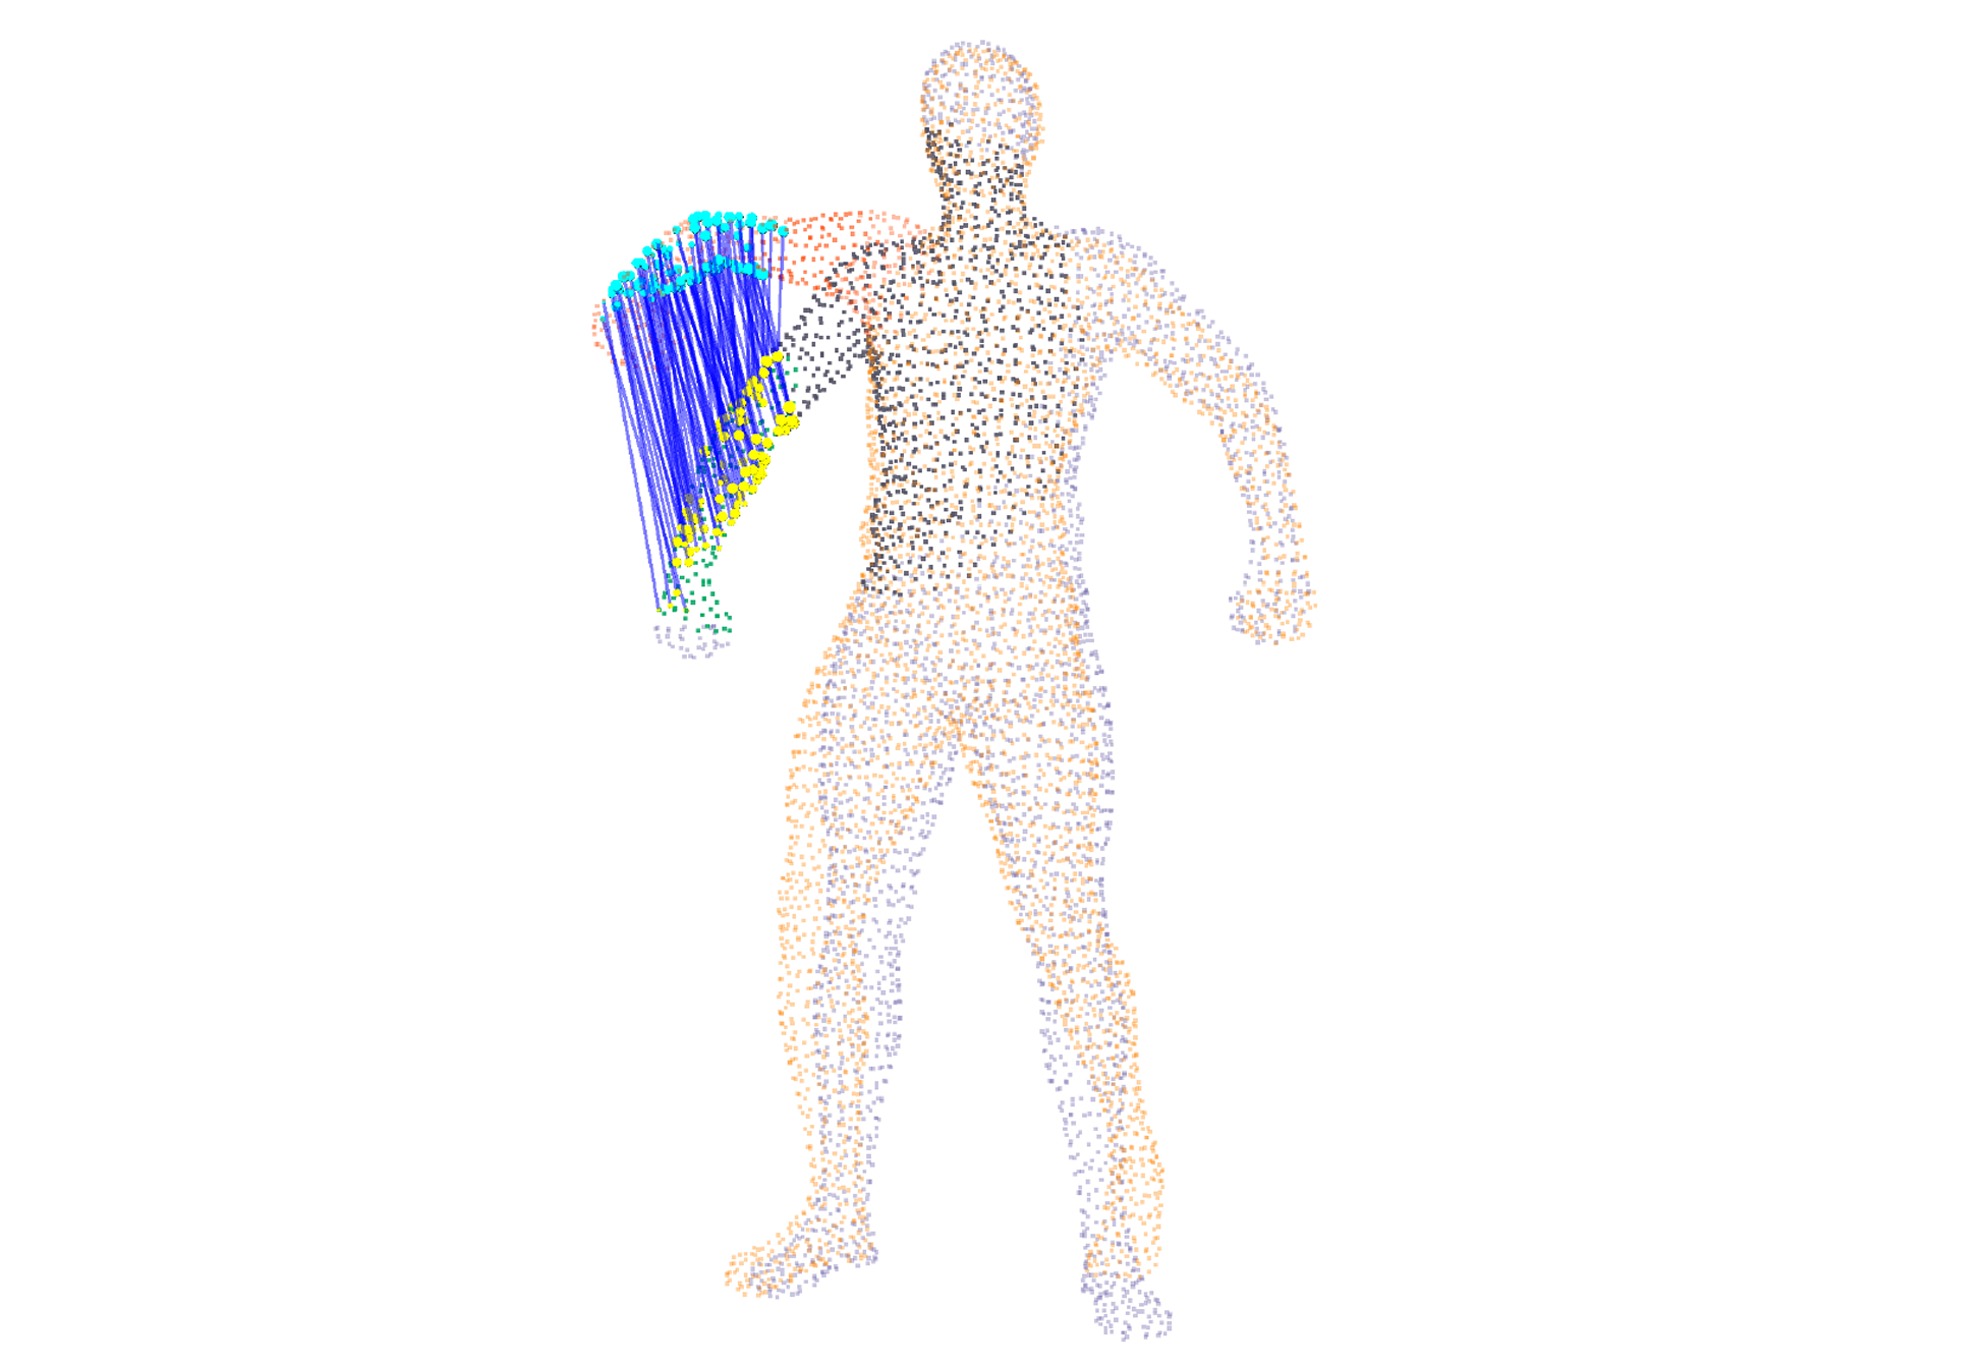
\includegraphics[width=0.45\textwidth]{LRP_arm}} 
		\\
		(a) & (b) 
	\end{tabular}
	\caption{Detecting the largest rigid part of an object~(a), and align the object to recursively detect linking parts to the LRP~(b) \cite{guo2016correspondence}.} 
	\label{fig:LRP_algorithm}
\end{figure}
%%
Another approach is achieved by Symmetrization \cite{Mitra07}, by detecting and aligning the body parts’ symmetry axes of an object(see figure \ref{fig:Symmetrization}). Based on Anguelov \cite{Anguelov04} and Mitra \cite{Mitra07}, Chang et al developed a closely related approach \cite{chang08articulated} \cite{chang09range}.
%%
\begin{figure}[H]
	\centering\small
	\begin{tabular}{cc}
		\fbox{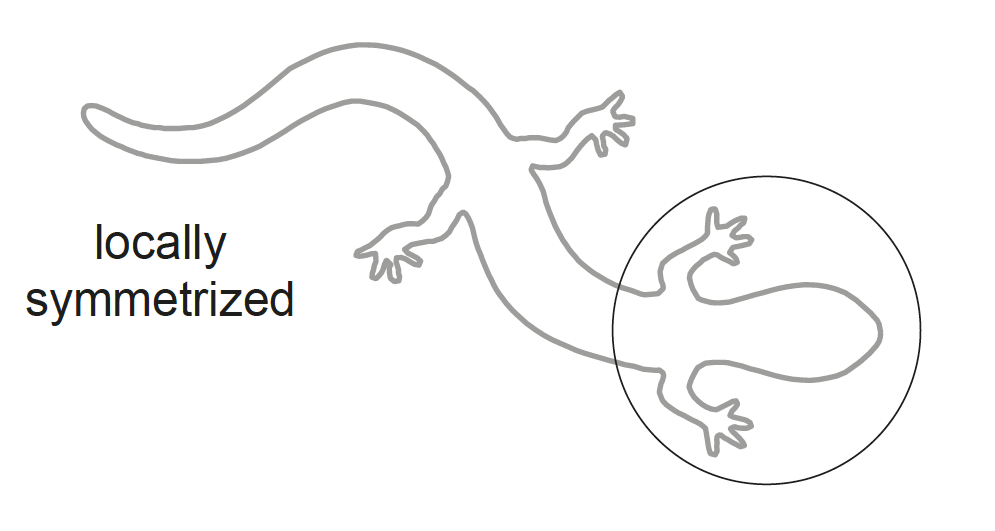
\includegraphics[width=0.45\textwidth]{Symmetrization1}} &
		\fbox{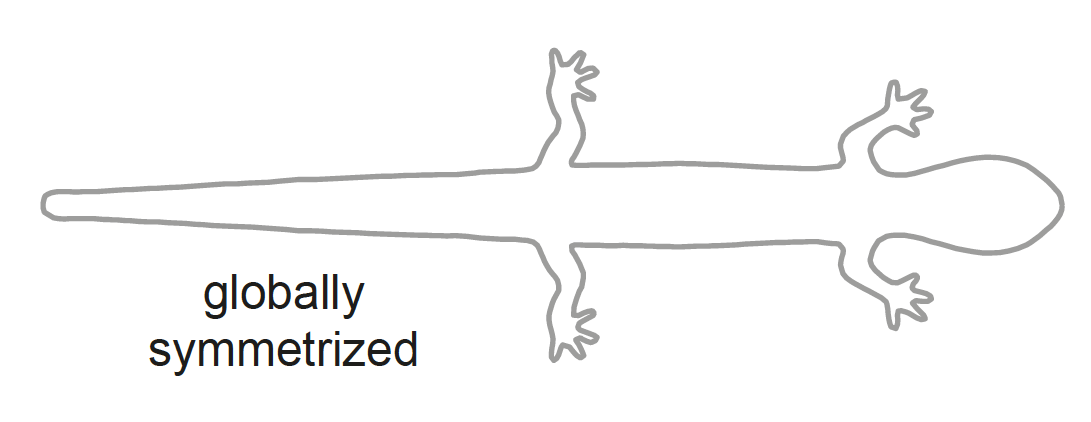
\includegraphics[width=0.45\textwidth]{Symmetrization2}} 
		\\
		(a) & (b) 
	\end{tabular}
	\caption{Detection of the rigid parts of an object by local~(a) and global~(b) Symmetrization \cite{Mitra07}.} 
	\label{fig:Symmetrization}
\end{figure}
%%

%TODO: Add other references
\subsection{Possible improvements}

%TODO: What are the main deficits of the algorithms?

The proposed approaches achieve convincing results concerning the accuracy of the segmentation and the detection of rigid parts. However, they are all computationally expensive and require a considerable number of computation steps to iteratively detect rigid parts in two associated objects. This reflects on the run time of the algorithm which offers therefore great potential for improvements.

Taking the existing methods as reference (see chapter \ref{cha:RelatedWork}) a new segmentation approach is developed. Thereby, the main focus is to reduce the computation steps of the correlated correspondence algorithm \cite{CorrelatedCorrespondance} as well as the LRP algorithm \cite {guo2016correspondence}. To fully focus on the segmentation into its rigid part, the 3D reconstruction of the articulated object is assumed to be available.

\section{Main Goal}

The goal is to segment an articulated mesh $M$ into its unknown number $n$ of rigid parts $\mathcal{P} =  \{P_1,\ldots,P_n\}$ and extract all joints $m$ $\mathcal{J} =  \{J_1,\ldots,J_m\}$ linking those parts in form of a skeleton structure. In general, this is done by non-rigid registration of the point clouds $C_1$ and $C_2$ of an object in two different poses. $C_1$ is thereby used as a \textit{template} to be registered with $C_2$. The main task is to determine a part assignment $P_i$ and the corresponding transformation $T_i$ for all points of the \textit{template} that aligns them with all points of $C_2$. Basically, a divide and conquer approach is implemented to recursively subdivide $C_1$ and $C_2$ into matching sub clusters. 

\section{Assumptions}

The input mesh $M$ is assumed to solely consist of rigid parts that can not be deformed or stretched (e.g. rigid parts of a human) and are linked by joints. Comparing two poses being adopted by the articulated object, the geodesic distance $g(\boldsymbol{p}_i,\boldsymbol{p}_j)$ between two mesh points $\boldsymbol{p}_i(x,y)$ and $\boldsymbol{p}_j(x,y)$ remains constant. Thereby, it is taken advantage of the knowledge that points located on a rigid part $P_i$ have the same transformation $T_i$ . Furthermore, it is assumed that the two poses of $M$ are oriented in the same direction.

\section{Chosen environment}

The initial approach was implemented in Java, using ImageJ as processing library. The chosen environment depends on the following factors:
\begin{itemize}
	\item familiarity and prior experience
	\item complexity
	\item available plug-in for image processing
\end{itemize}
%%
As ImageJ is mainly used for 2D use cases, another implementation would be possible in 3D using PCL in C++. As a result, the attention can be brought to segmentation and visualization in 3D.
